\section{搜索}
\subsection{基本搜索算法}
\subsubsection{树搜索算法和图搜索算法}
\begin{figure}[htbp]
    \centering
    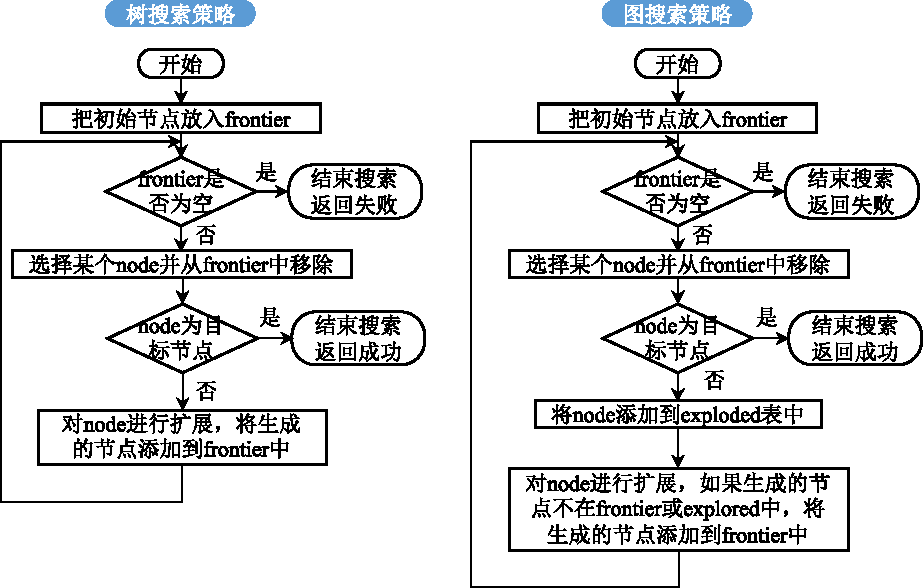
\includegraphics{image/图搜索和树搜索.pdf}
\end{figure}
\subsection{盲目搜素策略}
\begin{example}
    如图,$S$为初始状态,$G_1$和$G_2$为目标状态。忽略各状态之间的代价,注意连线是有方向的。在其他条件都相同的情况下,按照字母先后顺序对节点进行扩展。
    \begin{figure}[htbp]
        \centering
        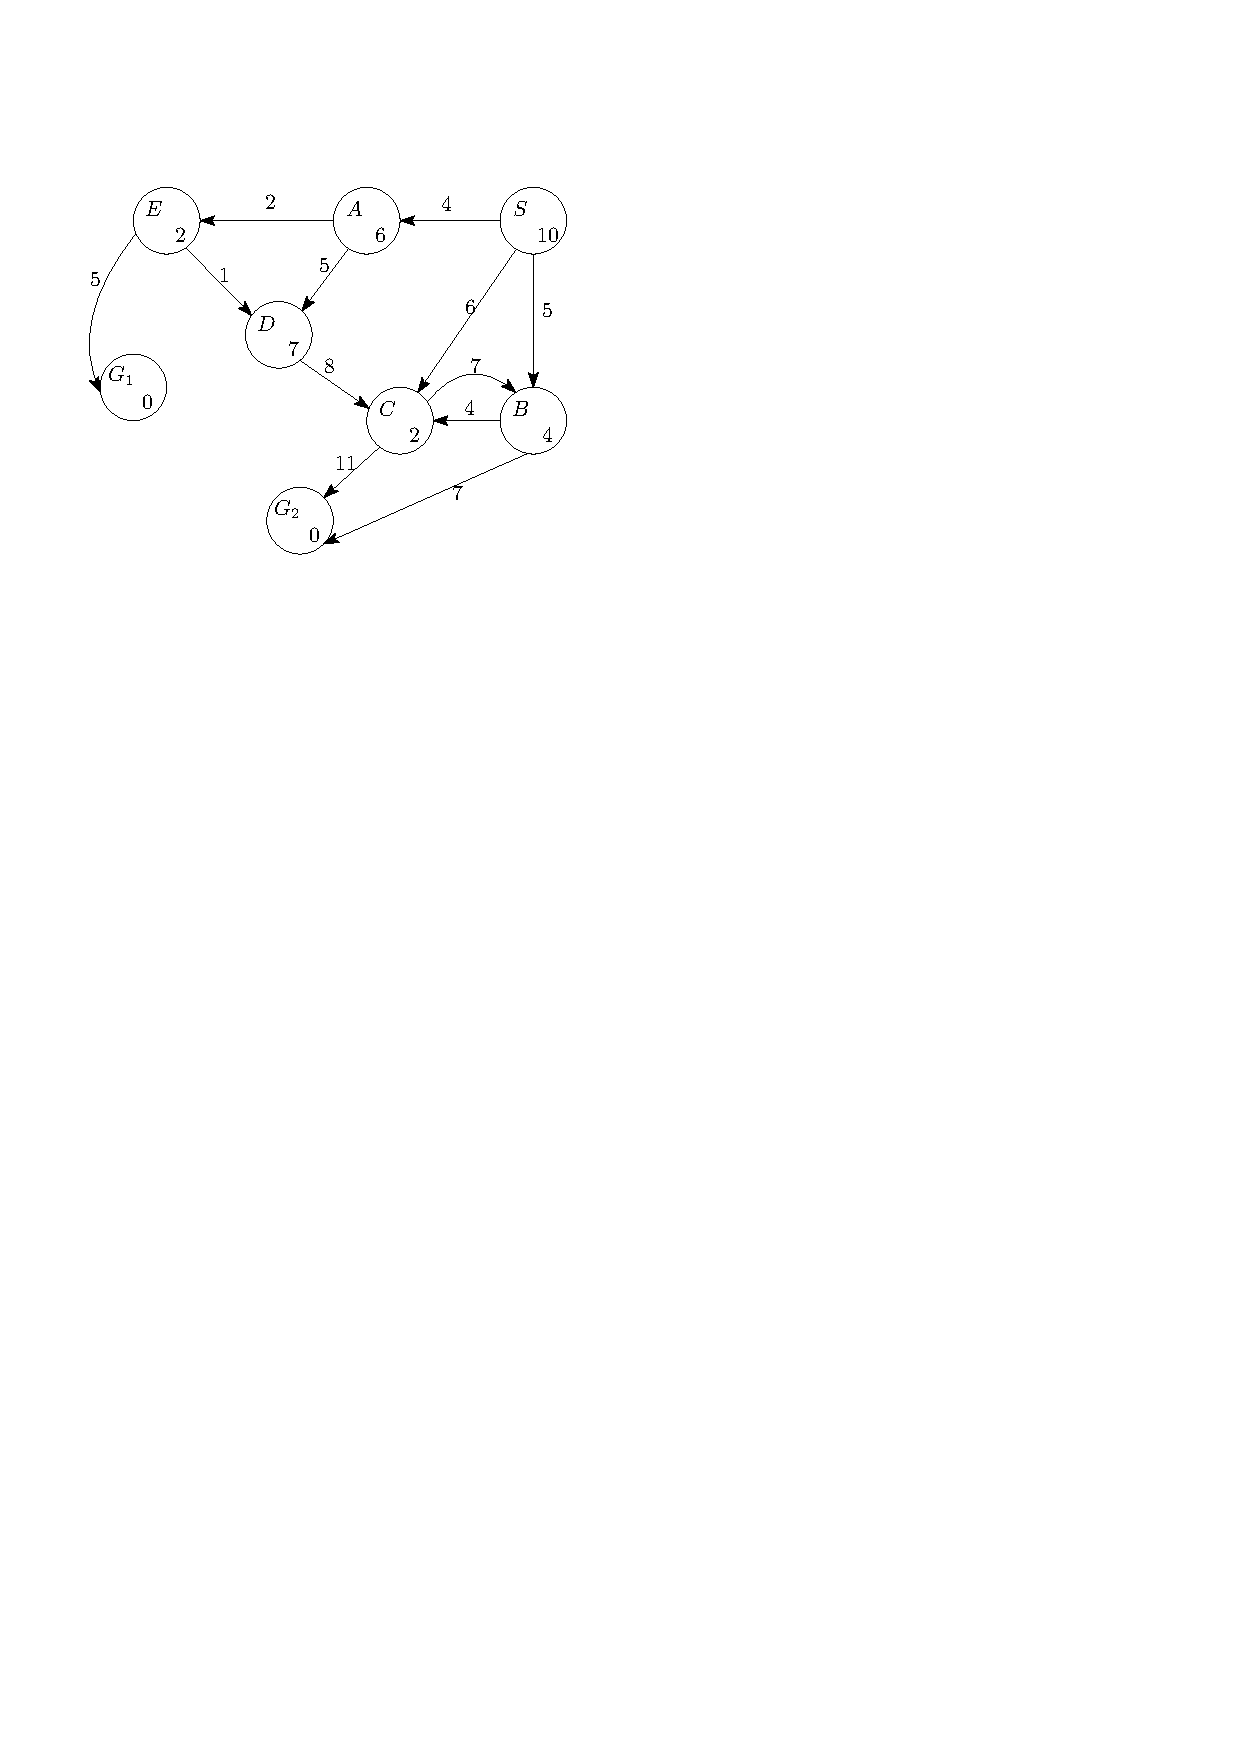
\includegraphics{image/搜索策略例题.pdf}
    \end{figure}
    \begin{enumerate}
        \item 应用\textcolor{main1}{宽度优先搜索}策略,指出\textcolor{main1}{树搜索}算法将会到达的目标状态,并按顺序写出搜索过程中所扩展出的节点。
        \item 应用\textcolor{main1}{宽度优先搜索}策略,指出\textcolor{main1}{图搜索}算法将会到达的目标状态,并按顺序写出搜索过程中所扩展出的节点。
    \end{enumerate}
    
    \textcolor{main1}{树搜索}:达到目标状态为$G_2$,解序列:$S\to B\to G_2$
    % Table generated by Excel2LaTeX from sheet '树搜索'
    \begin{table}[htbp]
        \centering
        \begin{tabular}{cc}
            \toprule[1.5pt]
            Step & frontier \\
            \midrule[1pt]
            Step 1 & $A,\, B,\, C$ \\
            Step 2 & $B,\, C,\, D,\, E$ \\
            Step 3 & $C,\, D,\, E,\, C,\, G_2$ \\
            Step 4 & $D,\, E,\, C,\, G_2,\, B,\, G_2$ \\
            Step 5 & $E,\, C,\, G_2,\, B,\, G_2,\, C$ \\
            Step 6 & $C,\, G_2,\, B,\, G_2,\, C,\, D,\, G_1$ \\
            Step 7 & $G_2,\, B,\, G_2,\, C,\, D,\, G_1,\, B,\, G_2$ \\
            \bottomrule[1.5pt]
        \end{tabular}%
    \end{table}%
  
    \textcolor{main1}{图搜索}:达到目标状态为$G_2$,解序列:$S\to B\to G_2$
    % Table generated by Excel2LaTeX from sheet '图搜索'
    \begin{table}[htbp]
        \centering
        \begin{tabular}{ccc}
        \toprule[1.5pt]
            Step & frontier & explored \\
            \midrule[1pt]
            Step 1 & $A,\, B,\, C$ & $S$ \\
            Step 2 & $B,\, C,\, D,\, E$ & $S,\, A$ \\
            Step 3 & $C,\, D,\, E,\, G_2$ & $S,\, A,\, B$ \\
            Step 4 & $D,\, E,\, G_2$ & $S,\, A,\, B,\, C$ \\
            Step 5 & $E,\, G_2$ & $S,\, A,\, B,\, C,\, D$ \\
            Step 6 & $G_2,\, G_1$ & $S,\, A,\, B,\, C,\, D,\, E$ \\
        \bottomrule[1.5pt]
        \end{tabular}%
    \end{table}%
\end{example}
\subsection{最佳优先搜索}
\subsubsection{评价函数}
\begin{definition}[评价函数]
    用来\textcolor{main1}{估算}经过节点$n$的路径代价的函数叫做\textcolor{main1}{评价函数},也称\textcolor{main1}{评估函数},用$f(n)$表示。
\end{definition}
\begin{note}
    路径的代价包括两部分:
    \begin{itemize}
        \item 一部分是确定性的代价。从起点到$n$的路径已经探索出来了,所耗费的代价可以精确计算,记为$g(n)$
        \item 一部分是不确定的代价。从$n$到终点的可能路径还没有探索出来,其代价只能进行预估,记为$h(n)$
    \end{itemize}
    \[
        f(n) = g(n) + h(n)
    \]
\end{note}
\subsubsection{一致代价搜索}
\begin{definition}[一致代价搜索]
    从初始状态到节点$n$已经产生的代价,\textcolor{main1}{无信息搜索策略}
    \[
        f(n) = g(n)
    \]
\end{definition}


\subsubsection{贪婪搜索}
\begin{definition}[贪婪搜索]
    贪婪搜索
    \[
        f(n) = h(n)
    \]
\end{definition}


\subsubsection{A\texorpdfstring{\textsuperscript{*}}{*}搜索}
\begin{definition}[A\textsuperscript{*}搜索]
    A\textsuperscript{*}搜索
    \[
        f(n) = g(n) + h(n)
    \]
\end{definition}

\begin{table}[htbp]
    \centering
    \resizebox{.95\textwidth}{!}{%
    \begin{tabular}{@{}cccc@{}}
    \toprule[1.5pt]
    搜索策略 & 一致代价 & 贪婪最佳优先 & A* \\ \midrule[1pt]
    评估函数 & $g(n)$ & $h(n)$ & $g(n)+h(n)$ \\
    完备性 & \begin{tabular}[c]{@{}c@{}}\textcolor{main1}{Yes*}:每步代价都>$\varepsilon>0$\\ 即无零代价步(图、树)\end{tabular} & \begin{tabular}[c]{@{}c@{}}\textcolor{main1}{树搜索}:否\\ 有限状态图搜索:是\end{tabular} & \multirow{2}{*}{\begin{tabular}[c]{@{}c@{}}$h(n)$若满足特定条件:\\ A*即完备且最优\end{tabular}} \\
    最优性 & \begin{tabular}[c]{@{}c@{}}\textcolor{main1}{Yes*}:比最优解代价小\\ 的节点数目优先(图、树)\end{tabular} & 否 &  \\
    时间复杂度 & $b^{1+[C^*/\varepsilon]}$ & \begin{tabular}[c]{@{}c@{}}$b^m$,\\ $m$搜索空间最大深度\end{tabular} & \multirow{2}{*}{\begin{tabular}[c]{@{}c@{}}扩展节点以解路径的长度呈指数增长。对于每\\ 步骤代价为常量的问题时间复杂度是最优解\\ 所在深度$d$的函数。\end{tabular}} \\
    空间复杂度 & $b^{1+[C^*/\varepsilon]}$ & \begin{tabular}[c]{@{}c@{}}$b^m$,\\ 保存所有节点在内存中\end{tabular} &  \\ \bottomrule[1.5pt]
    \end{tabular}%
    }
\end{table}
\begin{example}
    试用以下算法进行求解进行求解。
    \begin{figure}[H]
        \centering
        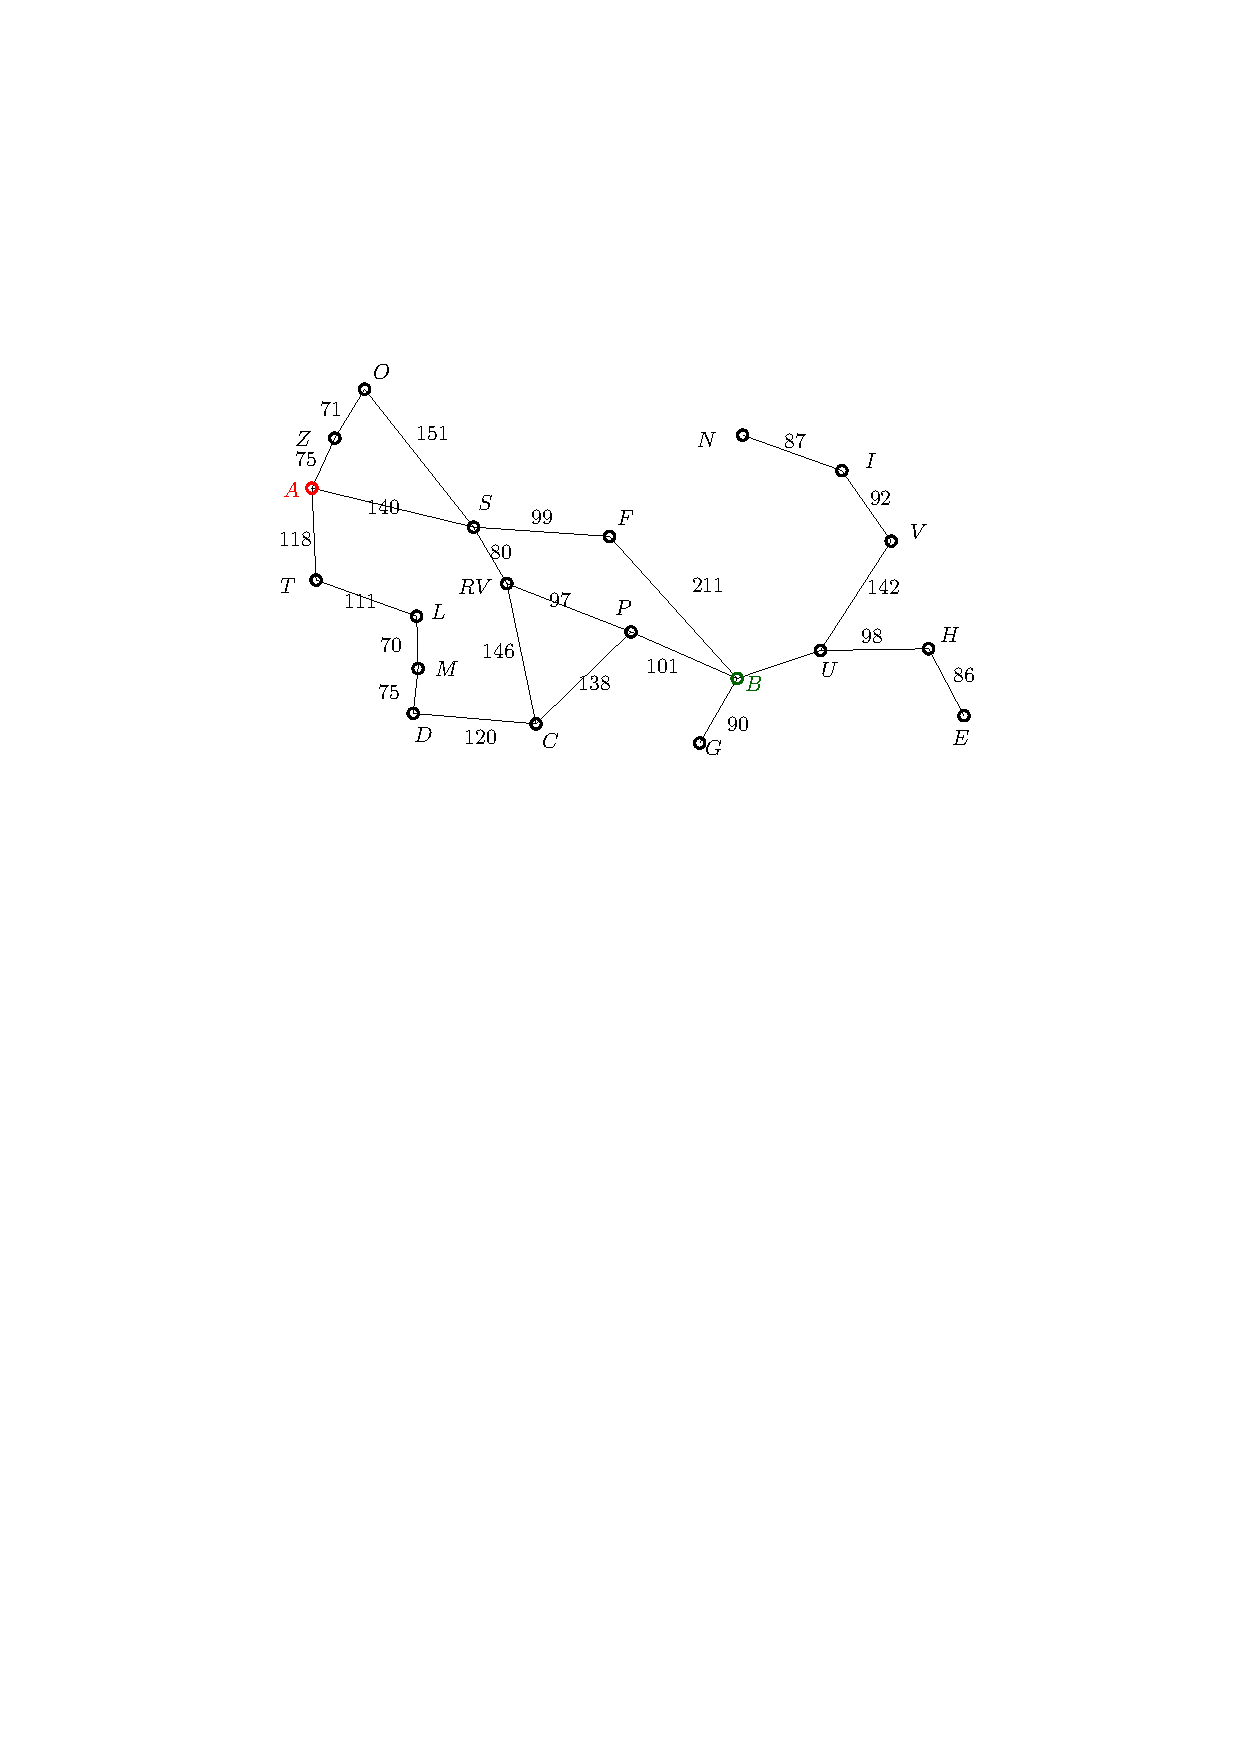
\includegraphics{image/评价函数例题.pdf}
    \end{figure}
    \begin{enumerate}
        \item 一致代价图搜索
        
        \textcolor{main1}{解序列:}$A\to S\to RV\to P\to B$

        \textcolor{main1}{解代价:}408
        % Table generated by Excel2LaTeX from sheet '一致代价搜索'
        \begin{table}[htbp]
            \centering
            \begin{tabular}{cc}
            \toprule[1.5pt]
            Step & frontier \\
            \midrule[1pt]
            Step 1 & $A(0)$ \\
            Step 2 & $Z(75),\,T(118),\,S(140)$ \\
            Step 3 & $T(118),\,S(140),\,O(146)$ \\
            Step 4 & $S(140),\,O(146),\,L(229)$ \\
            Step 5 & $O(146),\,RV(220),\,L(229),\,F(239)$ \\
            Step 6 & $RV(220),\,L(229),\,F(239)$ \\
            Step 7 & $L(229),\,F(239),\,P(317),\,C(366)$ \\
            Step 8 & $F(239),\,M(299),\,P(317),\,C(366)$ \\
            Step 9 & $M(299),\,P(317),\,C(366),\,B(450)$ \\
            Step 10 & $P(317),\,C(366),\,D(374),\,B(450)$ \\
            Step 11 & $C(366),\,D(374),\,B(408)$ \\
            Step 12 & $D(374),\,B(408)$ \\
            Step 13 & $B(408)$ \\
            \bottomrule[1.5pt]
            \end{tabular}%
        \end{table}%
        \item 贪婪搜索
                
        \textcolor{main1}{解序列:}$A\to S\to F\to B$

        \textcolor{main1}{解代价:}450
        \begin{figure}[H]
            \centering
            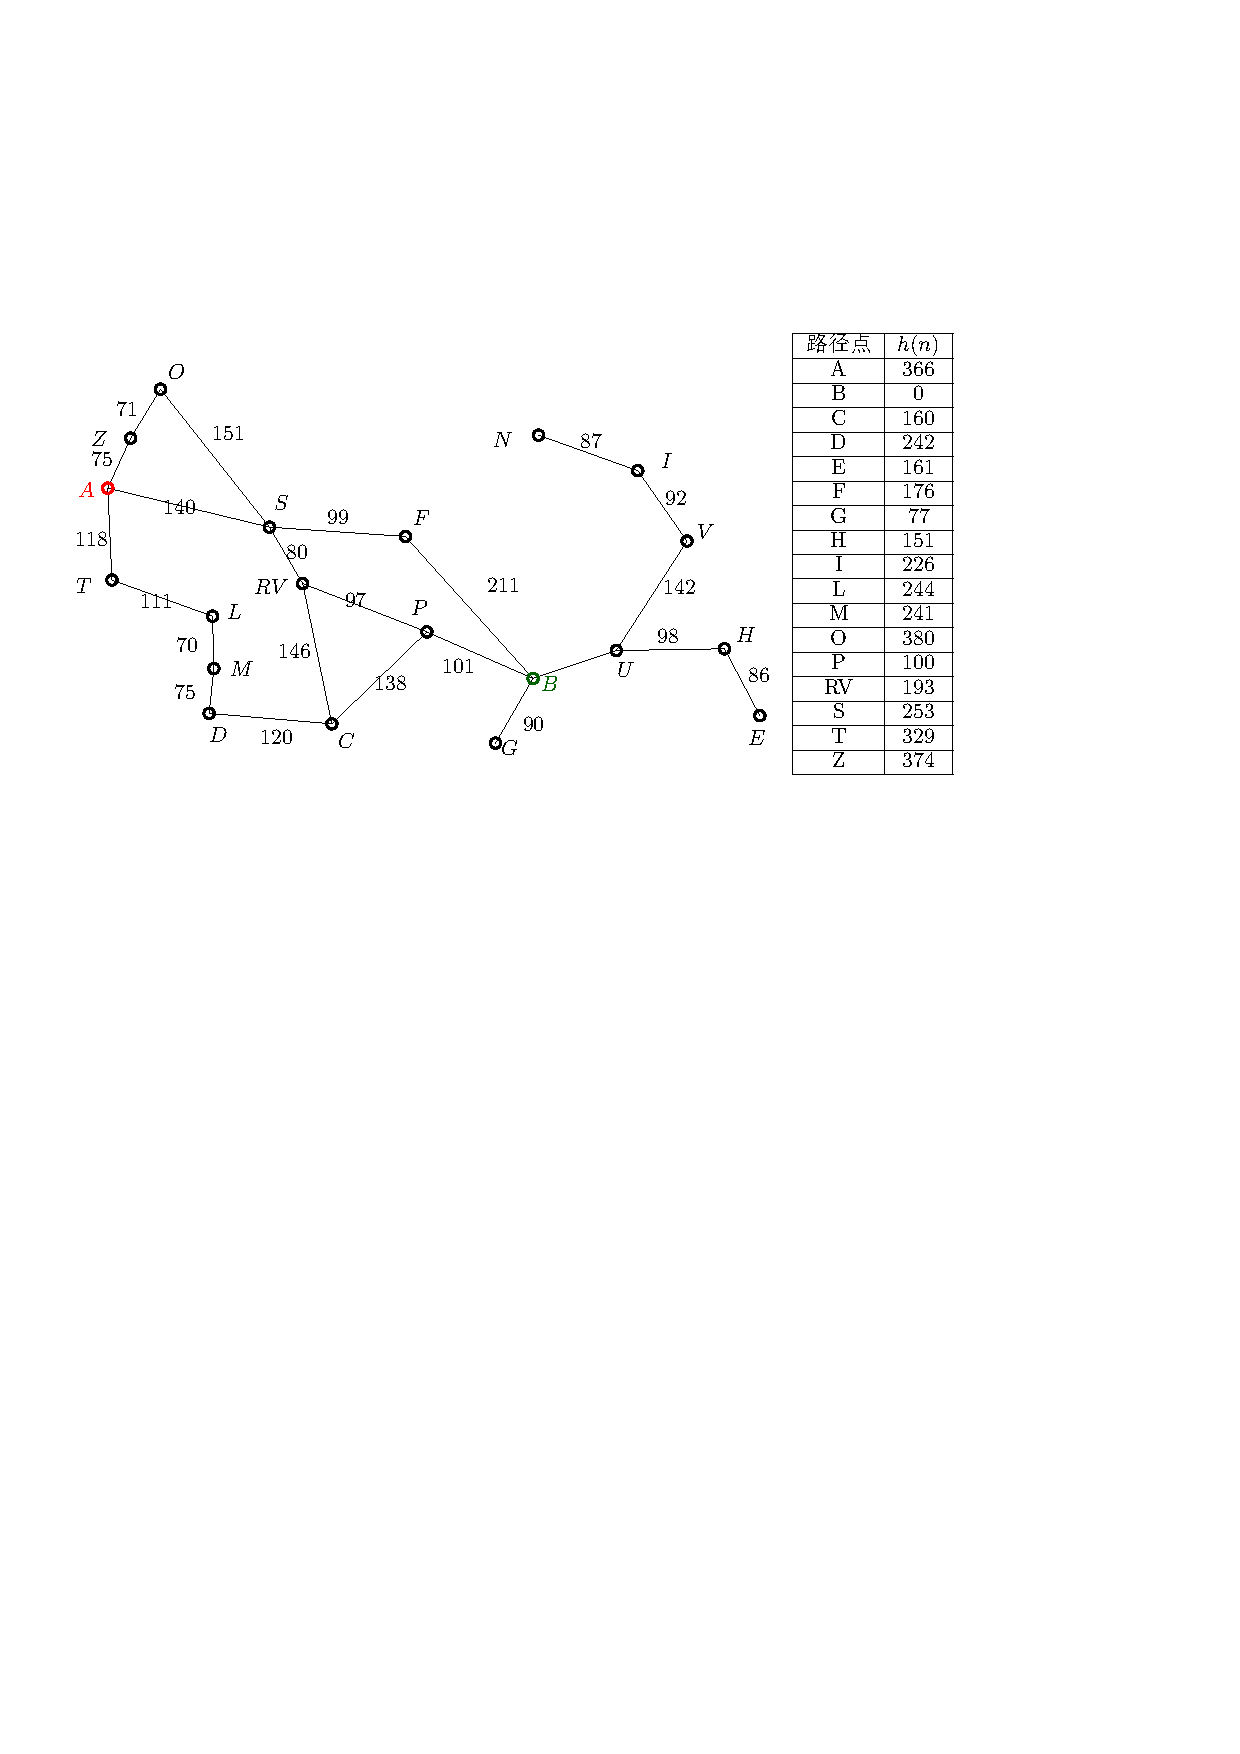
\includegraphics[width = \textwidth]{image/评价函数例题-1.pdf}
        \end{figure}
        % Table generated by Excel2LaTeX from sheet '贪婪搜索 (2)'
        \begin{table}[htbp]
            \centering
            \begin{tabular}{ccc}
            \toprule[1.5pt]
            Step & frontier & explored \bigstrut\\
            \midrule[1pt]
            Step 1 & $A(366)$ &  \bigstrut[t]\\
            Step 2 & $S(253),\,T(329),\,Z(374)$ & $A$ \\
            Step 3 & $F(176),\,RV(193),\,T(329),\,Z(374),\,O(380)$ & $A,\,S$ \\
            Step 4 & $B(0),\,RV(193),\,T(329),\,Z(374),\,O(380)$ & $A,\,S,\,F$ \bigstrut[b]\\
            \bottomrule[1.5pt]
            \end{tabular}%
        \end{table}%
        \item A\textsuperscript{*}搜索
        
        \textcolor{main1}{解序列:}$A\to S\to RV\to P\to B$

        \textcolor{main1}{解代价:}408
        % Table generated by Excel2LaTeX from sheet 'A-Star'
        \begin{table}[htbp]
            \centering
            \begin{tabular}{ccc}
            \toprule[1.5pt]
            Step & frontier & explored \\
            \midrule[1pt]
            Step 1 & $A(366)$ &  \\
            Step 2 & $S(393),\,T(447),\,Z(449)$ & $A$ \\
            Step 3 & $RV(413),\,F(415),\,T(447),\,Z(449),\,O(671)$ & $A,\,S$ \\
            Step 4 & $F(415),\,P(417),\,T(447),\,Z(449),\,C(526),\,O(671)$ & $A,\,S,\,RV$ \\
            Step 5 & $P(417),\,T(447),\,Z(449),\,B(450),\,C(526),\,O(671)$ & $A,\,S,\,RV,\,F$ \\
            Step 6 & $B(408),\,T(447),\,Z(449),\,C(526),\,O(671)$ & $A,\,S,\,RV,\,F,\,P$ \\
            \bottomrule[1.5pt]
            \end{tabular}%
        \end{table}%
    \end{enumerate}
\end{example}
\begin{example}
    $S$为初始状态,$G_1$和$G_2$为目标状态。各状态之间的代价已标注在连接两个状态的连线上 (注意连线是有方向的),每个状态到达目标的估计代价标注在其内部。分别应用\textcolor{main1}{一致代价、贪婪、A\textsuperscript{*}搜索策略},指出图搜索算法将会到达的目标状态($G_1$或$G_2$),并按顺序写出搜索过程中所考察的节点。在其他条件都相同的情况下,按照字母先后顺序对节点进行扩展。
    \begin{figure}[htbp]
        \centering
        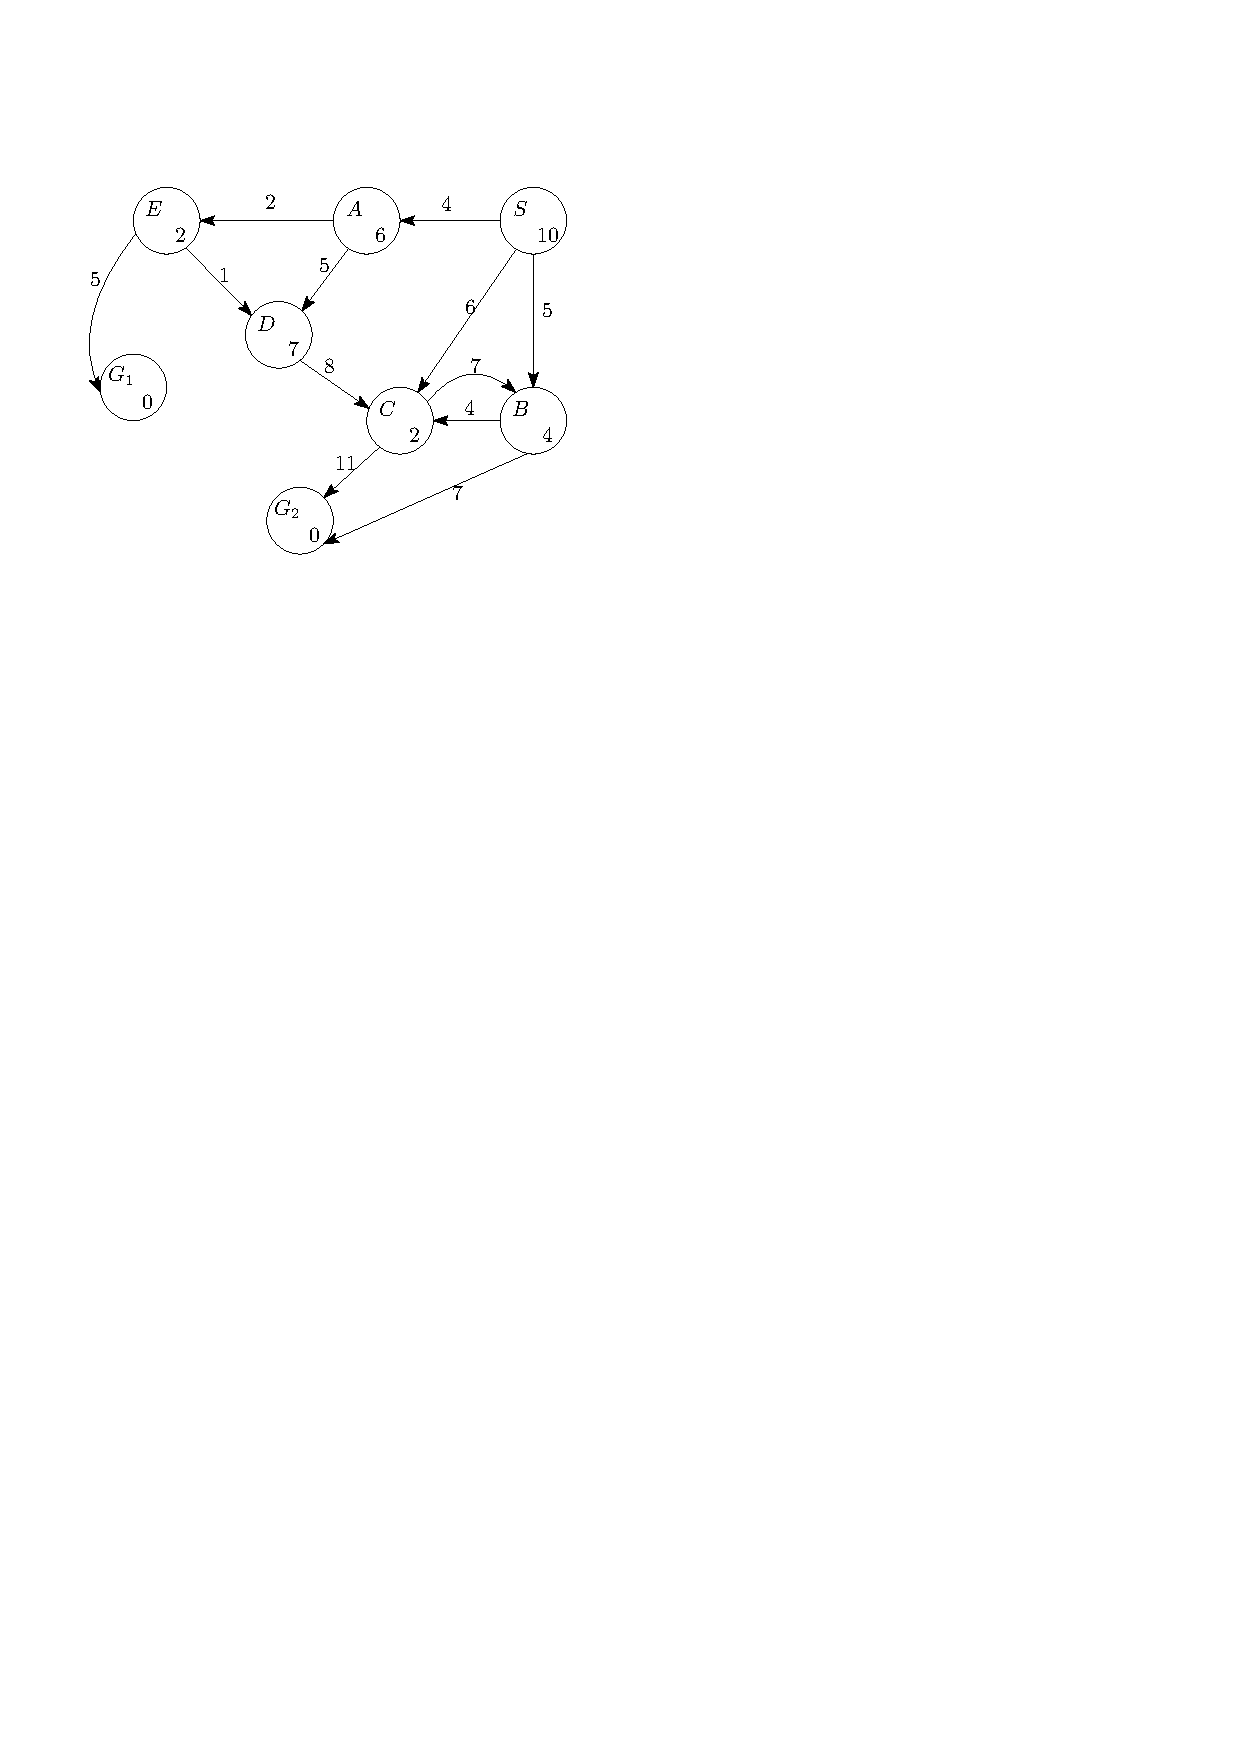
\includegraphics{image/搜索策略例题.pdf}
    \end{figure}
    \begin{enumerate}
        \item 一致代价
        
        \textcolor{main1}{解序列:}$S\to A\to E\to G_1$

        \textcolor{main1}{解代价:}11
        % Table generated by Excel2LaTeX from sheet '一致代价搜索'
        \begin{table}[htbp]
            \centering
            \begin{tabular}{ccc}
            \toprule[1.5pt]
            Step & frontier & explored \\
            \midrule[1pt]
            Step 1 & $S(0)$ &  \\
            Step 2 & $A(4),\,B(5),\,C(6)$ & $S$ \\
            Step 3 & $B(5),\,C(6),\,E(6),\,D(9)$ & $S,\,A$ \\
            Step 4 & $C(6),\,E(6),\,D(9),\,G_2(12)$ & $S,\,A,\,B$ \\
            Step 5 & $E(6),\,D(9),\,G_2(12)$ & $S,\,A,\,B,\,C$ \\
            Step 6 & $D(7),\,G_1(11),\,G_2(12)$ & $S,\,A,\,B,\,C,\,E$ \\
            Step 7 & $G_1(11),\,G_2(12)$ & $S,\,A,\,B,\,C,\,E,\,D$ \\
            \bottomrule[1.5pt]
            \end{tabular}%
        \end{table}%  
        \item 贪婪
                
        \textcolor{main1}{解序列:}$S\to C\to G_2$

        \textcolor{main1}{解代价:}17
        % Table generated by Excel2LaTeX from sheet '贪婪搜索 (2)'
        \begin{table}[htbp]
            \centering
            \begin{tabular}{ccc}
            \toprule[1.5pt]
            Step & frontier & explored \\
            \midrule[1pt]
            Step 1 & $S(0)$ &  \\
            Step 2 & $C(2),\,B(4),\,A(6)$ & $S$ \\
            Step 4 & $G_2(0),\,B(4),\,A(6)$ & $S,\,C$ \\
            \bottomrule[1.5pt]
            \end{tabular}%
        \end{table}%
        \item A\textsuperscript{*}
                        
        \textcolor{main1}{解序列:}$S\to A\to E\to G_1$

        \textcolor{main1}{解代价:}11
        % Table generated by Excel2LaTeX from sheet 'A-Star'
        \begin{table}[htbp]
            \centering
            \begin{tabular}{ccc}
            \toprule
            Step & frontier & explored \\
            \midrule
            Step 1 & $S(10)$ &  \\
            Step 2 & $C(8),\,B(9),\,A(10)$ & $S$ \\
            Step 3 & $B(9),\,A(10),\,G_2(12)$ & $S,\,C$ \\
            Step 4 & $A(10),\,G_2(12)$ & $S,\,C,\,B$ \\
            Step 5 & $E(8),\,G_2(12),\,D(16)$ & $S,\,C,\,B,\,A$ \\
            Step 6 & $G_1(11),\,G_2(12),\,D(14)$ & $S,\,C,\,B,\,A,\,E$ \\
            \bottomrule
            \end{tabular}%
        \end{table}%
    
    \end{enumerate}
\end{example}
\subsection{博弈树搜索}
\subsubsection{博弈问题}
\begin{definition}[博弈]
    在一定条件下,遵守一定的\textcolor{main1}{规则},\textcolor{main1}{一个或几个}拥有绝对理性思维的人或团队,从各自允许选择的行为或策略中选择并加以实施,并从中各自取得相应\textcolor{main1}{结果或收益}的过程。
\end{definition}
\begin{definition}[双方信息完备的零和博弈]
    包括以下内容:\newline
    \begin{itemize}
        \item 对抗的双方
        
        双方参与者轮流采取行动,选取对自己最有利而对对方最不利的对策
        \item 双方信息完备的零和博弈
        
        任何一方都了解当前的格局及过去的历史
        \item 零和
        
        参与者的利益严格对立,双方得失之和为零
    \end{itemize} 
\end{definition}

\begin{note}
    \textcolor{main1}{信息完备:}
    已知对方走过的棋步以及当前的局面。

    \textcolor{main1}{信息不完备:}
    参与人并不完全清楚对手的情况,只能进行估计。
\end{note}

\begin{example}
    下面哪些属于双方信息完备的零和博弈:
    \begin{enumerate}[A.]
        \item \textcolor{main1}{五子棋}
        \item 桥牌
        \item \textcolor{main1}{中国象棋}
        \item \textcolor{main1}{足球}
        \item \textcolor{main1}{围棋}
        \item 中美经济博弈
    \end{enumerate}
\end{example}

博弈问题分析的关键要素:
\begin{enumerate}
    \item 状态:棋盘上棋子位置布局
    \item 动作:各类棋子合法走步
    \item 开局/终局:游戏开始/结束的状态
    \item 终局效用值:终局下某个棋手的效用值
    \item 状态空间:合法动作作用于当前状态生成的博弈树
    \item 某个玩家的\textcolor{main1}{解}为一个\textcolor{main1}{策略}: 状态$\to $动作
\end{enumerate}
\subsubsection{minimax搜索算法}
极小极大搜索算法(三个阶段)
\begin{enumerate}
    \item 生成规定深度的全部博弈树,计算所有最底层节点的静态估计函数值
    \item 自底向上逐层计算非终结节点的倒推估计值
    \begin{itemize}
        \item 对于MAX层节点,取其所有子节点的最大值
        \item 对于MIN层节点,取其所有子节点的最小值
    \end{itemize}
    \item 标记最佳走步:
    \begin{itemize}
        \item 对于MAX选手,选择使其$f$值最大的走步
        \item 对于MIN选手,选择使其$f$值最小的走步
    \end{itemize}
\end{enumerate}

算法性质分析:
\begin{figure}[htbp]
    \centering
    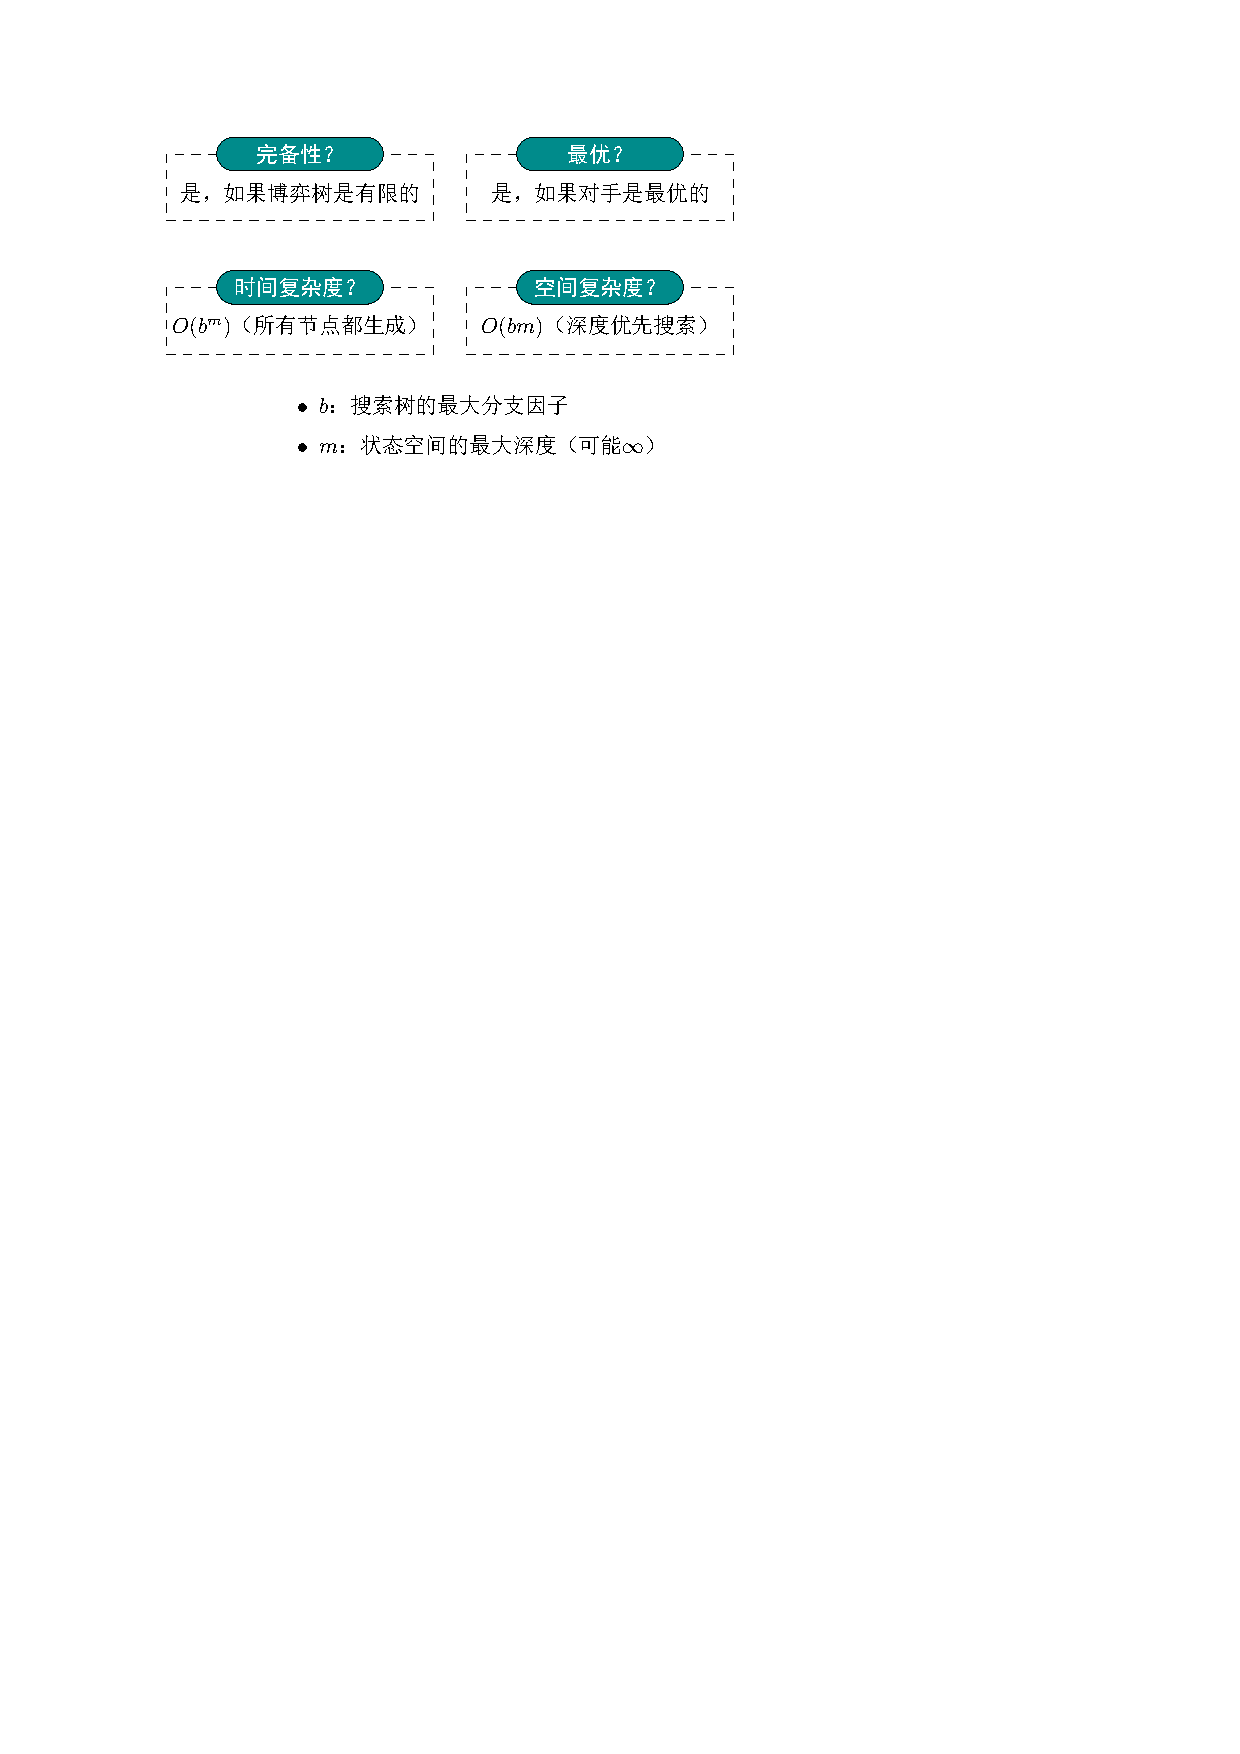
\includegraphics{image/minmax性质.pdf}
\end{figure}
\begin{note}
    博弈树的规模一般都很大
    \begin{itemize}
        \item 国际象棋:走10个会合后,总节点数量级$10^{31}$
        \item 中国象棋:走10个会合后,总节点数量级$10^{32}$
        \item 围棋:走10个回合后,总节点数量级$10^{51}$
    \end{itemize}
\end{note}
极大极小搜索过程存在的问题
由于要\textcolor{main1}{生成置顶深度以内的所有节点},其节点数将随着搜索深度的增加成指数增长。
\subsubsection{\texorpdfstring{$\alpha-\beta$}{α-β}剪枝}

\begin{note}
    进行$\alpha-\beta$剪枝时,应注意的问题
    \begin{itemize}
        \item 应\textcolor{main1}{相邻层比较}(MAX节点和MIN节点间),不能进行同层比较
        \item 至少一个子节点的推导值\textcolor{main1}{固定以后},才能向父节点传递
        \item 在实际搜索时,不能按宽度优先建立搜索树,再进行剪枝,而是按照\textcolor{main1}{有界深度优先搜索}的方式生成节点,\textcolor{main1}{边生成边剪枝}。
    \end{itemize}
\end{note}
\begin{note}
    特性分析
    \begin{itemize}
        \item $\alpha-\beta$剪枝对计算根节点的MiniMax值没有影响
        \item 剪枝效率最坏情况$O(b^m)$(其中$b$是分支数,$m$是解的深度)
        \item 剪枝效率最好情况$O(b^{m/2})$
        \begin{itemize}
            \item 不管是MAX选手还是MIN选手,最好选择都是博弈树的最左分枝,存在较多的剪枝。
        \end{itemize}
    \end{itemize}
\end{note}
\begin{example}
    对下面的博弈树按从左到右的顺序进行$\alpha-\beta$剪枝搜索,试标明各生成节点的倒推值,何处发生剪枝及应选择的走步。
    \begin{figure}[htbp]
        \centering
        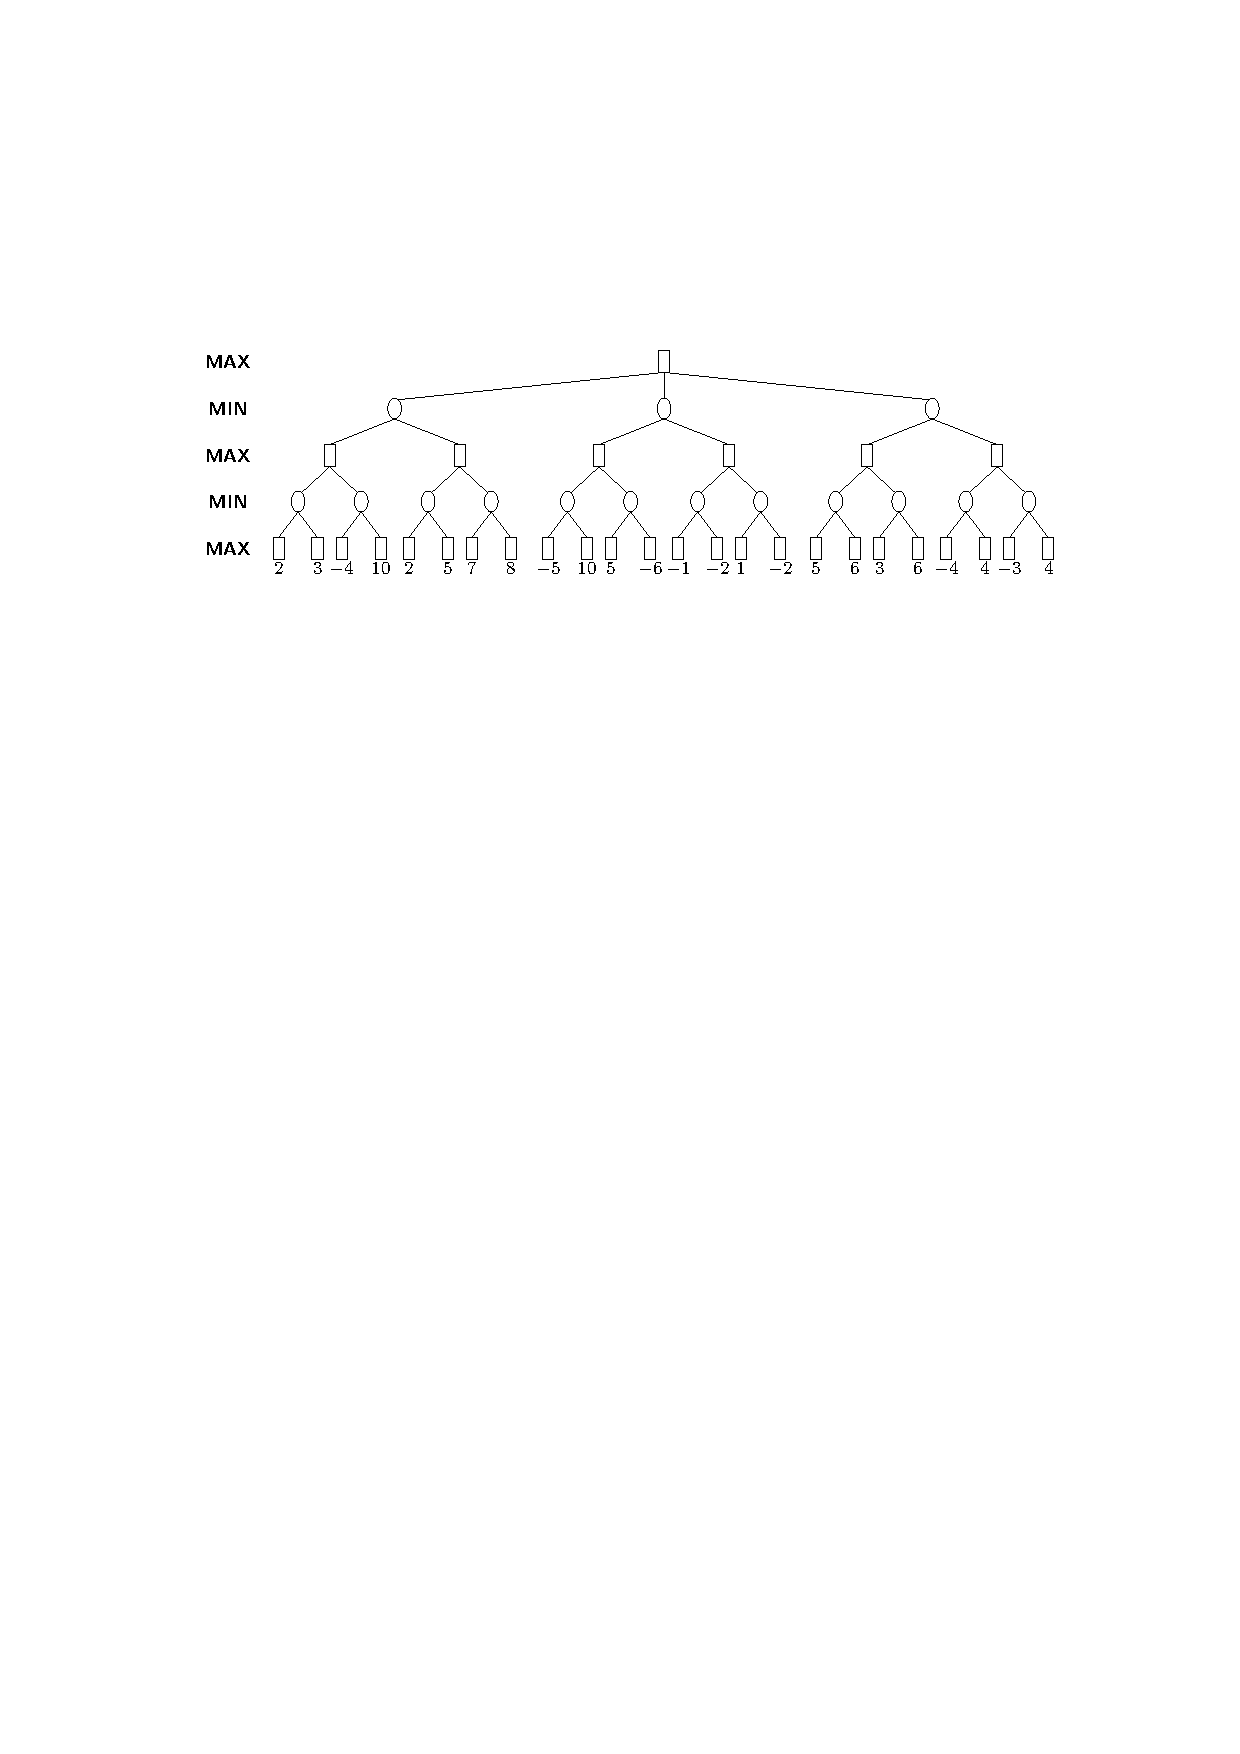
\includegraphics[width = .86\textwidth]{image/alpha-beta.pdf}
    \end{figure}

    \begin{figure}[htbp]
        \centering
        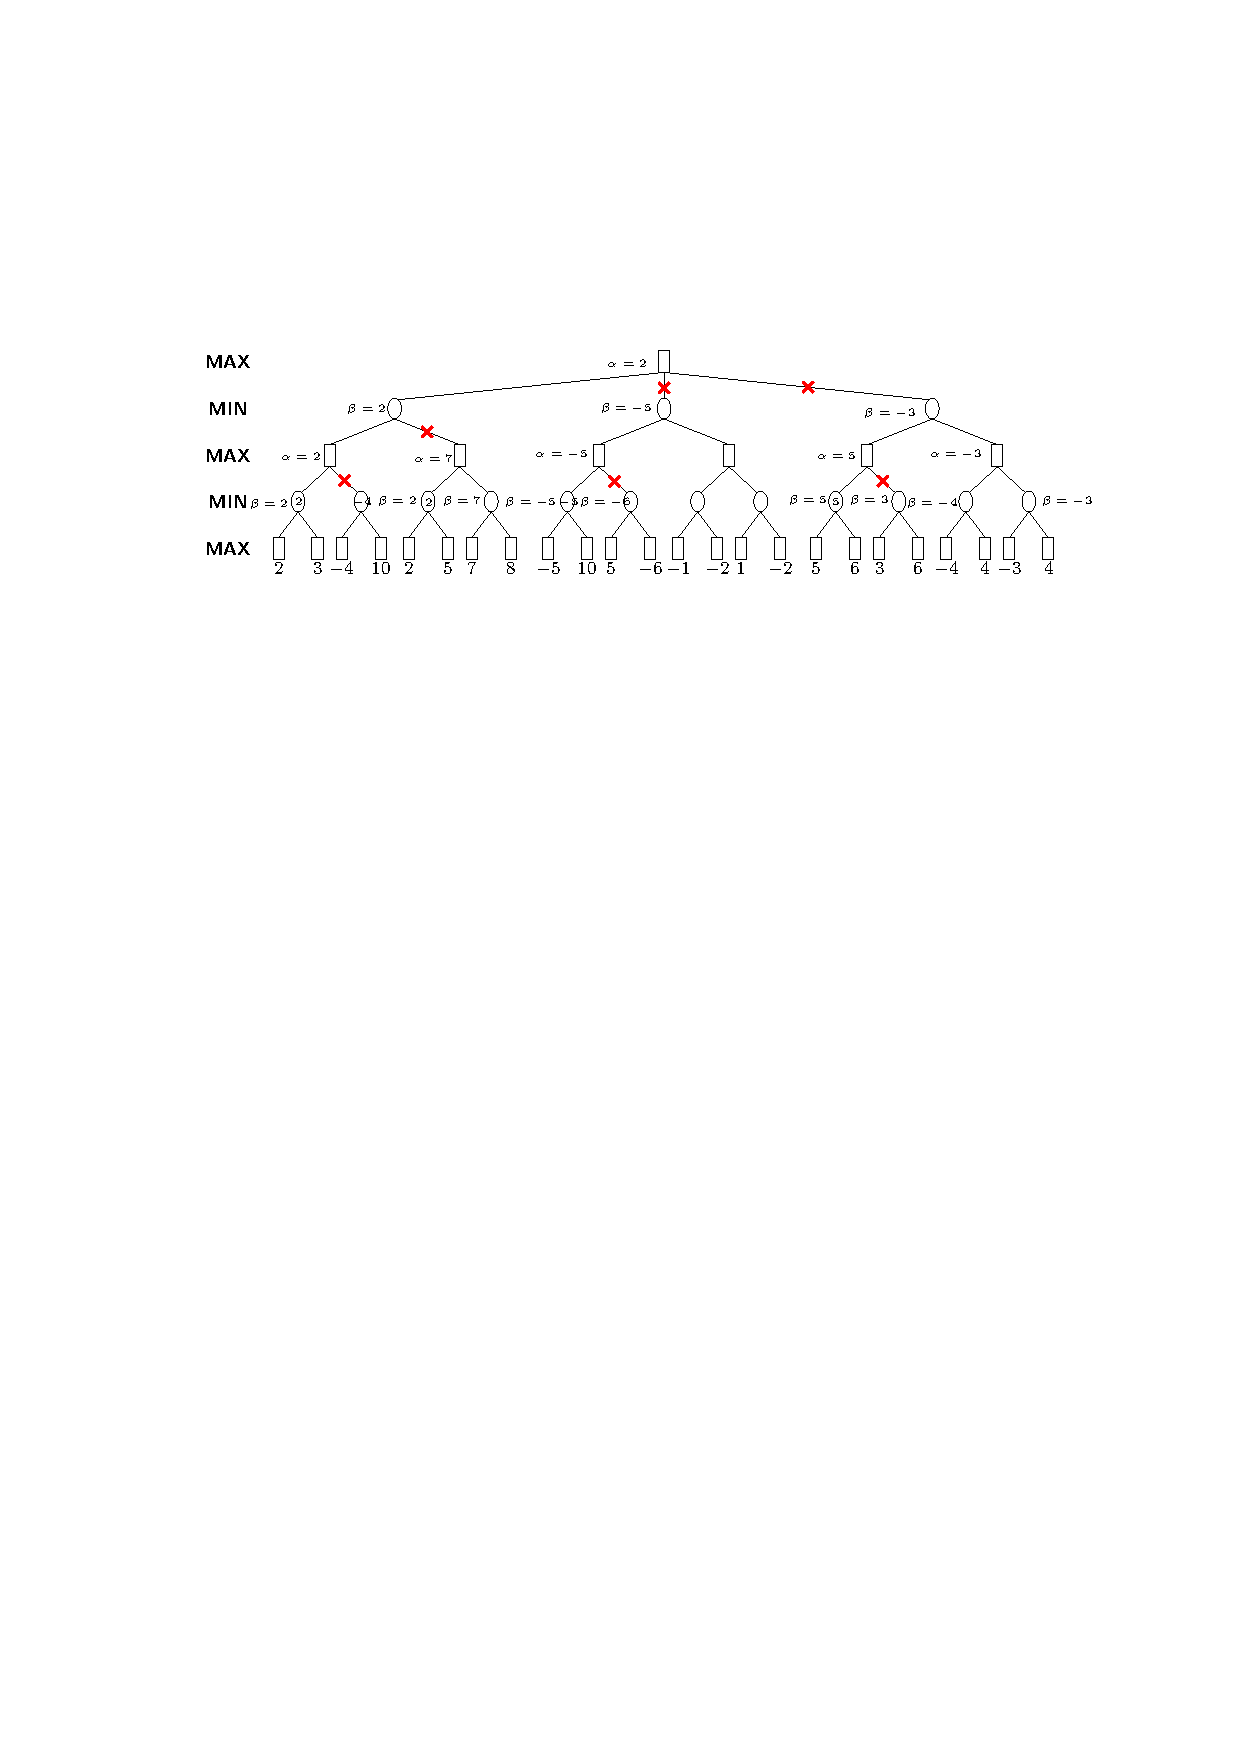
\includegraphics[width = .86\textwidth]{image/alpha-beta-sol.pdf}
    \end{figure}
\end{example}